\documentclass[aspectratio=169]{beamer}
\hypersetup{pdfpagemode=FullScreen}
\usetheme[progressbar=frametitle]{metropolis}
\usepackage{appendixnumberbeamer}
\usepackage{listings}
\bibliographystyle{plainnat}
\usepackage{listings}
\usepackage{hyperref}
\usepackage{booktabs}
\usepackage{tikz}
\usepackage{tikzpeople}
\usepackage{biblatex}
\addbibresource{references.bib}
\usetikzlibrary{shapes,arrows}
\usepackage[scale=1]{ccicons}
% \usepackage{enumitem} % not compatible with enumerate in beamer class
\usepackage{xspace}
\newcommand{\themename}{\textbf{\textsc{metropolis}}\xspace}

\title{Reddit Cryptocurrency Comments Analysis}
% \subtitle{Subtítulo}
% \date{\today}
\date{May 31, 2022}
\author{Albin Aliu, François-Xavier Wicht \& Grégoire Rebstein}
\institute{Social Media Analytics}
% \titlegraphic{\hfill\includegraphics[height=1.5cm]{logo.pdf}}

\begin{document}

\maketitle

\begin{frame}{Agenda}
    \setbeamertemplate{section in toc}[sections numbered]
    \tableofcontents
\end{frame}
\section{Overview}
\begin{frame}[t]
    \frametitle{Overview}
    \begin{columns}
        \column{0.4\textwidth}
        \begin{itemize}
            \item The main idea is to find a link between the activity in cryptocurrency subreddits and the price of \textbf{Bitcoin}.
            \item For that we modeled the data in an appropriate way and ran several algorithms seen in class.
        \end{itemize}
        %        \vspace{1.0cm}
        %        \includegraphics[width=0.8\textwidth]{figures/bitcoin_price.png}
        \column{0.5\textwidth}
        \includegraphics[width=0.8\textwidth]{figures/subreddits_labelled.png}
    \end{columns}
\end{frame}
\section{Trials and Errors}
\begin{frame}[t]
    \frametitle{Trials and Errors}
    The original idea was to perform Sentimental Analysis (SA) on Tweets.
    \vspace{2.0cm}
    \begin{columns}
        \column{0.5\textwidth}
        \begin{itemize}
            \item The Twitter API is unfortunately very limited.
            \item[$\implies$] We took Reddit as a Social Network instead.
        \end{itemize}
        \column{0.5\textwidth}
        \begin{itemize}
            \item Reddit is less suitable to perform Sentimental analysis.
            \item[$\implies$] We decided to analyse the network and find interesting results as well as correlation between subreddit's activity and Bitcoin price.
        \end{itemize}

    \end{columns}
\end{frame}
\section{Data collection}
\begin{frame}[t]
    \frametitle{Data collection}
    \vspace{1.0cm}
    \begin{columns}
        \column{0.4\textwidth}
        \begin{itemize}
            \item We used Reddit API for data collection.
            \item API calls are performed by a bot running every 20 minutes on several Cryptocurrency related subreddits.
            \item Storage is optimal in a JSON format because of Reddit comment structure.
        \end{itemize}
        \column{0.6\textwidth}
        \hspace{1.0cm}
        \includegraphics[width=0.5\textwidth]{figures/reddit_logo.png}
    \end{columns}
\end{frame}
\section{Data Models}
\newcounter{sauvegardeenumi}
\newcommand{\asuivre}{\setcounter{sauvegardeenumi}{\theenumi}}
\newcommand{\suite}{\setcounter{enumi}{\thesauvegardeenumi}}
\begin{frame}[t]
    \frametitle{Data Models}
    We have tried four types of data models.
    \begin{columns}
        \column{0.5\textwidth}
        \begin{enumerate}
            \item Unique Cartesian Link: all commenters from a specific post are linked together with an undirected edge.
            \item Deep Link: commenters are recursively linked together with a directed edge (i.e. capturing the relation ``has commented'') with a weight of relevance according to the depth of comments.
                \asuivre
        \end{enumerate}
        \column{0.4\textwidth}
        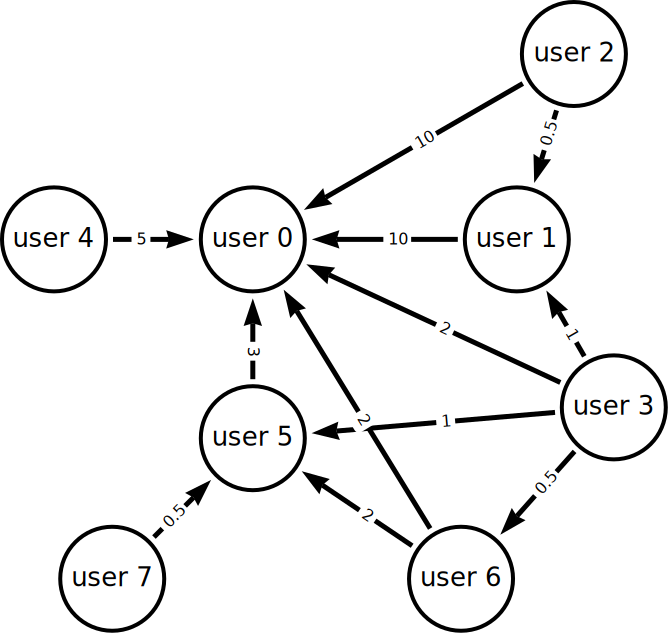
\includegraphics[width=0.8\textwidth]{figures/graph_model.png}
    \end{columns}
\end{frame}
\begin{frame}[t]
    \frametitle{Data Models}
    \vspace{1.0cm}
    \begin{columns}
        \column{0.6\textwidth}
        \begin{enumerate}
            \suite
            \item Next Link: only main commenters of the post are linked to the Original Poster (OP) with a directed edge.
            \item Deep Link No merge: same as Deep Link without merging the different edges. This results in a directed multigraph.
        \end{enumerate}
        \column{0.4\textwidth}
        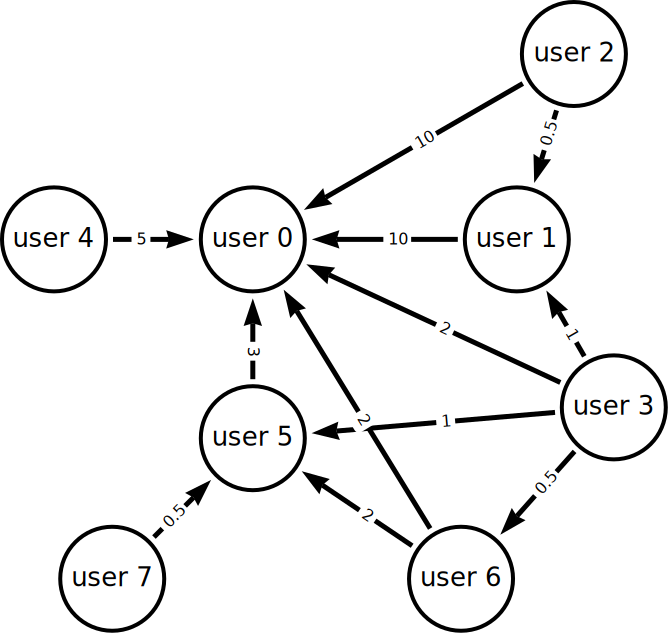
\includegraphics[width=0.8\textwidth]{figures/graph_model.png}
    \end{columns}
\end{frame}
\begin{frame}[t]
    \frametitle{Data Models}
    \vspace{1.0cm}
    \begin{columns}
        \column{0.4\textwidth}
        \begin{itemize}
            \item Deep Link No merge model represented on the right.
            \item Tree-like structure may be observed for large comments.
            \item Most imposing subreddits are Bitcoin, Dogecoin and Ethereum.
        \end{itemize}
        \column{0.6\textwidth}
        \includegraphics[width=0.7\textwidth]{figures/subreddits_labelled.png}
    \end{columns}
\end{frame}
\section{Analysis}
\begin{frame}[t]
    \frametitle{Power law distribution}
    \vspace{1.0cm}
    \begin{columns}
        \column{0.6\textwidth}
        \begin{itemize}
            \item The graph data model follows a Power law distribution.
            \item This most likely means that the data model is well thought out.
        \end{itemize}
        \column{0.4\textwidth}
        \includegraphics[width=\textwidth]{figures/deg_dist.pdf}
    \end{columns}
\end{frame}
\begin{frame}[t]
    \frametitle{PageRank}
    \begin{columns}
        \column{0.4\textwidth}
        \begin{itemize}
            \item The PageRank in the network can be interpreted as being the probability of commenting one user's post when browsing the given subreddits.
            \item Yet, the PageRank alone does not yield very surprising results: users with the most upvoted and commented comments have the highest PageRank.
        \end{itemize}
        \column{0.6\textwidth}
        \includegraphics[width=0.9\textwidth]{figures/rank_days.png}
    \end{columns}
\end{frame}
\begin{frame}[t]
    \frametitle{PageRank}
    \begin{columns}
        \column{0.6\textwidth}
        \begin{itemize}
            \item We therefore took interest in evaluating the \textbf{steadiness} of the PageRank along the days.
            \item We concluded two things.
                \begin{enumerate}
                    \item There is a tiny similarity between user bases along the days. Two days do not have a lot of users in common. 
                    \item There is a tiny error between PageRank intersections. Two days share about the same PageRank values for the same users.
                \end{enumerate}
            \item These two observations help us conclude that the topics and posts are lasting in time and this is consistent with other works \cite{glenskiCharacterizingSpeedScale2019, liMultiwindowBitcoinPrice2021}.
        \end{itemize}
        \column{0.5\textwidth}
        \includegraphics[width=0.6\textwidth]{figures/sim_days.pdf}
        \includegraphics[width=0.6\textwidth]{figures/error_days.pdf}
    \end{columns}
\end{frame}
\begin{frame}[t]
    \frametitle{Correlation to price development}
    \begin{columns}
        \column{0.5\textwidth}
        \begin{itemize}
            \item We made an inclusion sequence of graph with a time window of 1h.
                $$G_1\subset G_2\subset G_3\subset \ldots\subset G_n$$
            \item We used degree centrality to compare each Graph $i$ with its subsequent graph $i+1$.
            \item We match these data with the ones of the Bitcoin price rate.
            \item We applied some smoothing with the window average method.
        \end{itemize}
        \column{0.5\textwidth}
        \includegraphics[width=0.8\textwidth]{figures/activity_x_price.pdf}
        \includegraphics[width=0.8\textwidth]{figures/pearson.pdf}
        \begin{itemize}
            \item The correlation we've found is of $-0.85$.
        \end{itemize}
    \end{columns}
\end{frame}
\begin{frame}[t]
    \frametitle{Causal link}
    \vspace{1.0cm}
\begin{itemize}
    \item Yet, correlation does not capture causal link.
    \item Causal link is difficult to assess between activity in subreddits and price rate.
    \item \citetitle{wooleyExtractingCryptocurrencyPrice2019} shows with Granger causality tests, that there exists indeed a causal link between the two.
    \item Correlations have also been proven in \citetitle{iderCryptocurrencyReturnPrediction2022}.
\end{itemize}
\end{frame}
\begin{frame}[t]
    \frametitle{Louvain community detection method}
    
\end{frame}
\section{Homemade implementation}
\begin{frame}[t]
    \frametitle{PageRank}
    \begin{columns}
        \column{0.4\textwidth}
        \begin{enumerate}
            \item \citetitle{hagbergExploringNetworkStructure2008} and homemade implementation yields the same results.
            \item Yet, the benchmarks show a night and day difference.
            \item Using a dense matrix is the main reason behind that.
            \item It is a direct consequence of the Power Law distribution.
        \end{enumerate}
        \column{0.6\textwidth}
        \begin{table}[ht!]
            \centering
            \begin{tabular}{|l|l|l|l|l|} 
                \hline
                \tiny implementation & nodes & edges & time  & RAM     \\ 
                \hline
                \tiny NetworkX      & 15537 & 58150 & 0.78s & 0.128G  \\ 
                \hline
                \tiny homemade (dense)       & 15537 & 58150 & 91.21s   & 5.81G   \\
                \hline
            \end{tabular}
        \end{table}
    \end{columns}

\end{frame}
\begin{frame}[t]
    \frametitle{PageRank}
    \vspace{2.0cm}
    \begin{table}[ht!]
        \centering
        \begin{tabular}{|l|l|l|l|l|} 
            \hline
            implementation & nodes & edges & time  & RAM     \\ 
            \hline
            NetworkX      & 15537 & 58150 & 0.78s & 0.128G  \\ 
            \hline
            homemade (dense)       & 15537 & 58150 & 91.21s   & 5.81G   \\
            \hline
            homemade (sparse)      & 15537 & 58150 & 2.18s   & 0.215G   \\
            \hline
        \end{tabular}
        \caption{Benchmarks of PageRank algorithm on Fedora Linux 36 with Intel i7-8550U (8) @ 4.000GHz and 16GB of RAM}
    \end{table}
\end{frame}
\begin{frame}[t]
    \frametitle{Louvain}
\end{frame}
\section{Discussion}
\begin{frame}[t]
    \frametitle{Questions}
    \vspace{2.0cm}
    \begin{center}
        Any questions?
    \end{center}
\end{frame}
\begin{frame}[plain,allowframebreaks]
    \frametitle{References}
    \printbibliography

\end{frame}
\end{document}
